\chapter{Tecnologias}

Durante o desenvolvimento desse projeto utilizando o algoritmo NEAT, se fez 
necessário o entendimento, além do algoritmo em si, das tecnologias que o compõem,
sendo elas: Algoritmo Genético e Redes Neurais. 

Essas duas tecnologias quando combinadas de maneira harmoniosa e 
seguindo as bases teóricas presentes no NEAT, propiciam a melhor abstração do 
algoritmo em si.

\section{Algoritmo Gen{\'e}tico}

O processo evolutivo no campo da biologia é definido por
\citeonline{ridley2009evolucao} como uma mudança na forma e
nos comportamentos de uma determinada espécie ao longo das
gerações por um processo de seleção natural, “onde o indivíduo
mais bem adaptado sobrevive e deixa mais descendentes do que o
menos adaptado, o que conduz ao declínio de sua variedade ou
espécie, eventualmente conduzindo-a à extinção”
\cite{do2009alfred}.

A ideia de um AG é trazer todos esses conceitos embutidos na
biologia para modelos computacionais capazes de solucionar
problemas complexos de otimização por métodos
meta-heurísticos. Tais algoritmos não possuem um regra de
produção para seu desenvolvimento e implementação, sendo
apenas necessário abstrair a teoria biológica para o universo
da computação. Porém, de acordo com
\citeonline{mitchell1998introduction}, algumas
características, por convenção, sempre estão presentes, como,
por exemplo: populações de indivíduos, seleção dos mais aptos,
cálculo de função \textit{fitness}, \textit{crossovers} para a reprodução e
mutações aleatórias.

\subsection{Indiv{\'i}duo e popula{\c c}{\~a}o}

Com base nas informações supracitadas é possível destrinchar
cada característica para melhor entendimento, iniciando pelo
elemento base do AG, o indivíduo.

Cada indivíduo de uma população é composto por uma sequência
de cromossomos. Cada cromossomo é composto por um conjunto de
valores binários. Cada valor binário desse conjunto é chamado
de gene. Baseando-se nisso, é possível concluir que cada
indivíduo possui sua forma e comportamento ditados pelo seu
respectivo cromossomo e uma população é composta por um
conjunto de \textit{n} diferentes cromossomos, como pode ser visto na
\autoref{fig_gene}.

\begin{figure}[htb]
        \centering
        \caption{\label{fig_gene}Gene, Cromossomo e População.}
        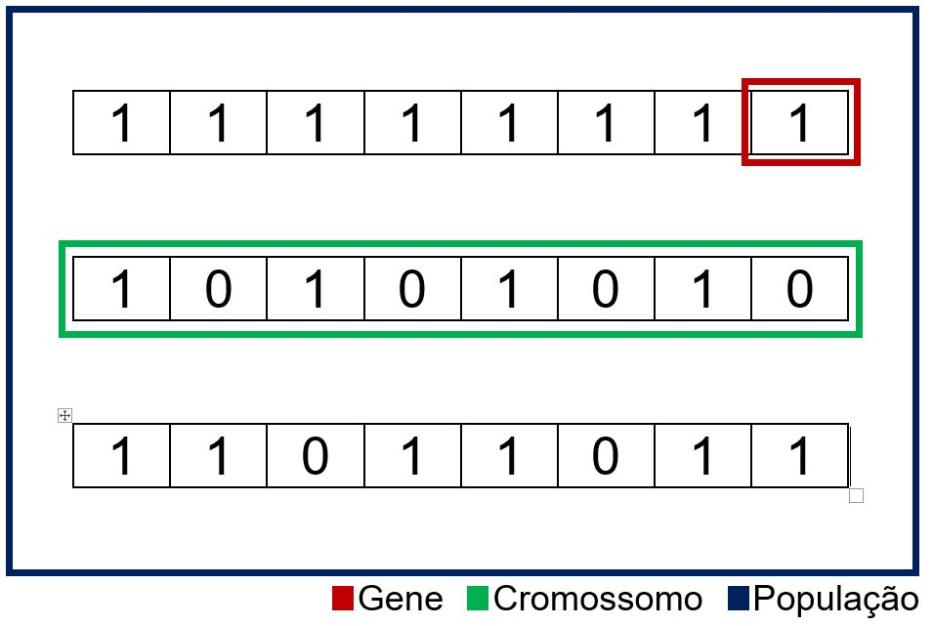
\includegraphics[width=0.7\textwidth]{images/gene.jpg}
        \legend{
                Fonte: Autoria Pr{\'o}pria.
        }
\end{figure}

\subsection{Reprodu{\c c}{\~a}o}

A reprodução é a parte considerada mais importante de um AG. É
nela que acontece a seleção e o cruzamento de cromossomos da
população com o intuito de gerar a evolução dos indivíduos e,
dessa forma, atingir o melhor resultado para a situação. 

Esse processo de reprodução é feito em etapas e ocorre sempre
que uma geração completa um ciclo de execução preestabelecido
e há a necessidade de se criar uma nova geração. Esse processo
de reprodução somente chega ao fim quando o resultado gerado
pelo AG atinge o valor esperado, ou por uma condição de parada
definida anteriormente. 

Referente às etapas que constituem a reprodução, estão
inclusos os operadores de seleção, \textit{crossover} e
mutação.

\subsubsection{Sele{\c c}{\~a}o}

A etapa de seleção leva em consideração uma função chamada
\textit{fitness}, que é única para cada indivíduo de cada
geração após a execução de um ciclo. O cálculo desta função
varia e é definida de acordo com o problema que o AG está
inserido, utilizando dados essenciais para que seja possível
classificar que um cromossomo obteve um bom desempenho em uma
determinada situação. 

Com a \textit{fitness} de cada indivíduo calculado, “o
operador seleciona os cromossomos da população para a
reprodução, quanto maior o valor da função \textit{fitness}, maior a
chance desse mesmo cromossomo ser selecionado mais vezes para
reprodução” \cite{mitchell1998introduction}.  Além dos
indivíduos com melhor \textit{fitness}, são selecionados também, de
maneira aleatória, os demais cromossomos, para que a chance de
chegar em máximo local seja reduzida. A quantidade de
indivíduos selecionados, assim como a proporção de reprodução,
deve ser minimamente suficiente para que a geração seguinte
possua o mesmo tamanho da anterior.

\subsubsection{\textit{Crossover}}

O \textit{crossover} é o responsável por gerar a evolução propriamente
dita. É durante essa etapa que os indivíduos recebem
características novas, porém, não necessariamente melhores.
Como dito anteriormente, o AG é um algoritmo meta-heurístico,
ou seja, busca otimizar problemas que não possuem
necessariamente apenas um resultado bom, mas sim diversos
resultados bons. Essa classificação se dá pelo “fato dos
cromossomos serem tratados apenas como sequências de bits sem
que sejam feitas inferências a respeito dos seus significados”
\cite{paulino2018}. Por isso, cromossomos anteriormente bons
podem perder suas qualidades e obter resultados piores na
geração seguinte, porém, a vantagem é que o contrário também é
verdadeiro. Cromossomos ruins podem ganhar qualidades e
obterem resultados melhores.

Essas trocas de características e cruzamentos entre
cromossomos é o que se chama de \textit{crossover}. A maneira com a qual o
\textit{crossover} é desenvolvido varia de acordo com a
situação em que o AG está inserido. Uma das maneiras mais
simples de realizar o \textit{crossover} é pegar dois cromossomos, ou
seja, duas cadeias binárias e realizar a inversão da primeira
metade do primeiro cromossomo com a segunda metade do segundo
cromossomo, como demonstrado na \autoref{fig_crossover}.

\begin{figure}[htb]
        \centering
        \caption{\label{fig_crossover}\textit{Crossover} entre dois cromossomos.}
        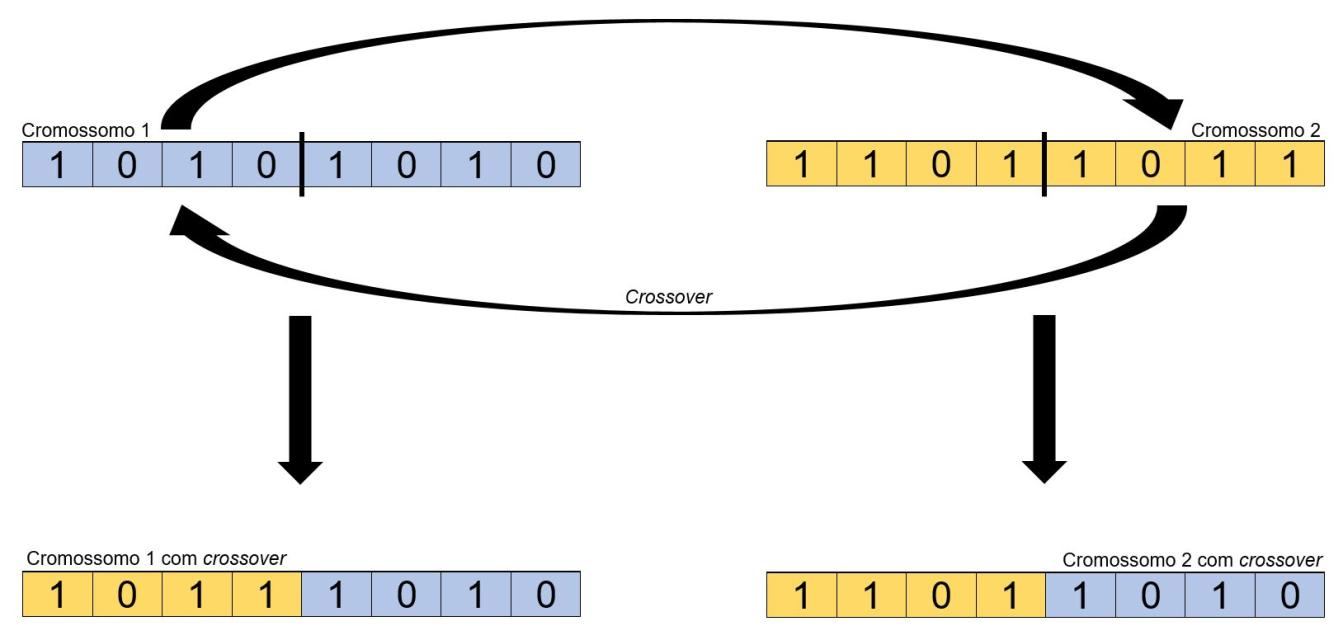
\includegraphics[width=0.7\textwidth]{images/crossover.jpg}
        \legend{
                Fonte: Autoria Pr{\'o}pria.
        }
\end{figure}

Dessa maneira ambos os cromossomos se beneficiam, ou não, das
características do outro sem perder todas as suas próprias
características. Esse processo cria uma nova população, porém,
as características da geração anterior, por mais que
distribuídas entre os cromossomos, ainda estão presentes, só
organizadas de maneira diferente, não tendo uma evolução
propriamente dita, para isso que a próxima etapa, mutação, se
faz necessária.

\subsection{Muta{\c c}{\~a}o}

Após o \textit{crossover}, a nova população possui cromossomos
com genes organizados de maneira diferente. A mutação entra
para gerar uma alternância nos genes dos cromossomos
selecionados aleatoriamente com o intuito de gerar novas
características para a população. Porém, apesar de útil, a
mutação deve ser utilizada com cautela, tanto na questão de
cromossomos selecionados para mutação, quanto na quantidade de
genes selecionados por cromossomo, para que não haja
alterações descontroladas e nada produtivas para a resolução
do problema.

\section{Redes Neurais}

Uma Rede Neural é uma abstração computacional baseada no 
funcionamento do sistema nervoso dos animais capaz de resolver problemas 
complexos com ou sem supervisão pertencente ao campo de IA. Esse sistema é 
composto por diversos neurônios e conexões entre esses mesmos neurônios para 
que sejam enviados sinais com comandos para as demais células do organismo 
vivo. A capacidade de tomada de decisão advém da organização dos neurônios e 
suas conexões formando uma grande e complexa rede onde a menor unidade que 
pode ser encontrada é o neurônio \cite{rojas2013neural}.

Um neurônio funciona recebendo informações fornecidas por demais neurônios,
gerando uma saída própria baseada nessas mesmas informações. No universo
computacional, o modelo com o objetivo de simular tais características de um
neurônio é chamado de \textit{perceptron}.

\subsection{\textit{Perceptron}}

Um \textit{perceptron} funciona recebendo e somando entradas \(x\) multiplicadas por 
um peso \(w\) correspondente junto com uma entrada de valor 1 sempre presente 
multiplicada por uma constante \(\theta\) chamada de viés. Esse somatório gera uma saída 
\textit{s} que pode ser expressa por \(s = \theta + xw\) e que passa por uma função de ativação 
que suaviza a curva de saída. Nesse projeto será utilizada a função de ativação 
\(tanh\), gerando então a saída \(s = tanh( \theta + xw)\). Uma visualização gráfica de tal 
estrutura pode ser encontrada na \autoref{fig_perceptron}.

\begin{figure}[htb]
        \centering
        \caption{\label{fig_perceptron}Estrutura b{\'a}sica de um \textit{perceptron}.}
        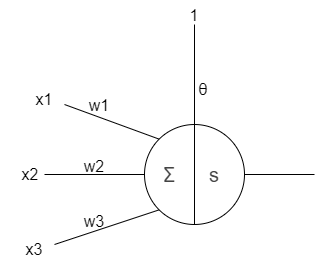
\includegraphics[width=0.7\textwidth]{images/Perceptron.png}
        \legend{
                Fonte: Autoria Pr{\'o}pria.
        }
\end{figure}

{\'E} no \textit{perceptron} que as decisões são tomadas, porém, para que se tenha a 
característica de malha que a Rede requer, interações entre \textit{perceptrons} se fazem 
necessárias, com cada \textit{perceptron} possuindo diferentes pesos e métricas definidos 
pelos resultados de saída de outros \textit{perceptrons}.

\subsection{\textit{Perceptrons} em m{\'u}ltiplas camadas}

Quando um \textit{perceptron} se associa a outros, através das diversas conexões 
entre si, a estrutura de Rede Neural propriamente dita começa a se formar. Essas 
mesmas conexões entre os \textit{perceptrons} são separadas em 3 camadas: de entrada, 
ocultas e de saída.

A camada de entrada tem como objetivo receber as informações do meio 
externo, e, posteriormente, abastecer a primeira camada oculta com estes mesmos 
dados. Cada \textit{perceptron} da primeira camada oculta recebe a saída de todos os 
\textit{perceptrons} da camada de entrada, como pode ser visto na \autoref{fig_camadasOocultas}.

\begin{figure}[htb]
        \centering
        \caption{\label{fig_camadasOocultas}Conex{\~o}es dos \textit{perceptrons} da Camada de Entrada com a primeira Camada Oculta.}
        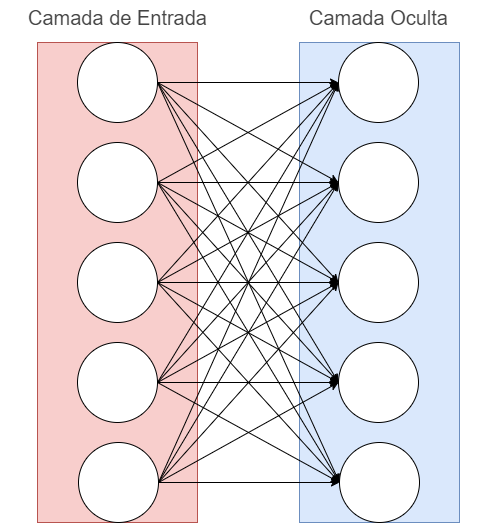
\includegraphics[width=0.7\textwidth]{images/CamadasOcultas.png}
        \legend{
                Fonte: Autoria Pr{\'o}pria.
        }
\end{figure}

O nome de camada oculta se dá pelo fato de que os valores das arestas de 
conexão são desconhecidos, sendo visíveis somente as entradas e as saídas ao final 
do processamento. A precisão obtida depende do número de \textit{perceptrons} utilizados 
nas camadas ocultas, sendo dentro das camadas ocultas que acontece o 
processamento bruto dos dados recebidos da camada de entrada \cite{liu2008uso}, 
onde o alto grau de comunicação dos \textit{perceptrons} gera diversos resultados 
que são avaliados por outros \textit{perceptrons} antes de serem encaminhados para a 
camada de saída. A maneira com a qual uma camada oculta se comporta é definida 
durante a modelagem das camadas e, também, o treinamento da Rede Neural com 
um conjunto de dados confiável, como será esclarecido na próxima seção.

Ao final, a camada de saída coleta os valores da última camada oculta, os 
interpreta e depois os expõe como resultados obtidos com base nas entradas.

\subsection{Treinamento}

O treinamento de uma Rede Neural se dá alimentando a mesma com uma 
base de dados previamente conhecida para que se possua controle dos valores de 
saída com base nas entradas. Uma das maneiras de tratar a base de dados no 
treinamento da Rede é utilizar o método de validação cruzada, onde, por exemplo,
uma base de dados de tamanho 100 tenha 80\% de seus valores utilizados para 
efetivamente treinar a Rede, com a mesma se balizando ao olhar suas próprias 
respostas e os 20\% dos dados restantes sendo utilizados para simular um ambiente 
real, onde a Rede exprime uma resposta com base nas entradas apenas. 

O conceito de se auto balizar da Rede pode ser dados por diversos 
algoritmos com funcionamentos e finalidades diferentes, porém, para esse projeto, 
será exposto o algoritmo chamado de \textit{backpropagation}. 

\subsubsection{\textit{Backpropagation}}

De acordo com \citeonline{rojas2013neural}, o algoritmo utiliza de fórmulas matemáticas, 
como o gradiente descendente, para calcular erros e diminuir a disparidade nas 
respostas de saída da Rede. Durante o processo de \textit{perceptrons}, a cada 
resposta, a Rede redistribui os pesos w nas arestas dos \textit{perceptrons} necessários 
em um movimento que parte da camada saída, passando pelas camadas ocultas e 
chegando até a camada de entrada, alterando também o viés de cada um para que 
seja então possível obter posteriormente uma resposta melhor e mais precisa. Esse 
processo vai então ensinando a Rede como se comportar em diferentes situações.

O backpropagation pode ser dividido em duas fases: a fase de cálculo de erro 
e a fase de redistribuição dos novos pesos aos \textit{perceptrons}. Durante a primeira 
etapa, utilizando o gradiente, a Rede verifica qual a resposta foi obtida e o quão 
distante a mesma está do resultado esperado, com esse valor é possível gerar uma 
função de propagação responsável por corrigir os pesos nas arestas, assim como o 
viés de cada \textit{perceptron}, e aproximar o resultado gerado pela Rede do resultado 
real esperado. Na segunda etapa, a Rede se encarrega de pegar essa função de 
propagação e ir aplicando a mesma nas camadas da Rede, de trás para frente, 
sendo por isso o nome do algoritmo, porém, essa função de propagação não é a 
mesma para todas as camadas. 

Com a função implementada na camada de saída, por exemplo, é possível 
calcular que valor a última camada oculta precisaria ter para chegar no valor 
necessário na camada de saída. É feito então um cálculo de uma nova função de 
propagação que é aplicada as arestas de tal camada. Esse mesmo processo é 
repetido de camada em camada, até que se chegue na primeira camada. Após todo 
esse processo, a Rede está com os pesos e o viés de cada \textit{perceptron} mais 
precisos.

De maneira mais abstraída, cada \textit{perceptron} possui uma resposta que é 
baseada em demais respostas de outros \textit{perceptrons} e também um viés próprio 
para aquela situação. Com o \textit{backpropagation}, cada \textit{perceptron} observa o quão 
errado ele estava e o quão errado estavam os resultados que o mesmo se baseou. 
Com essa correção, em uma nova situação problema,  seu viés é outro, assim como 
a probabilidade de considerar o resultado proveniente de um outro \textit{perceptron}.

\section{Neuroevolu{\c c}{\~a}o de Topologias Aumentantes}

Neuroevolução é a combinação de Redes Neurais e Algoritmos Genéticos, 
onde os cromossomos são representações compactas de Redes Neurais, que por 
sua vez são avaliadas pela função de aptidão \cite{stanley2004neat}. As peculiaridades 
do NEAT, de maneira prática, não partem do mesmo, mas sim da maneira com qual 
o Algoritmo Genético e as Redes Neurais são configurados. 	

\subsection{Bases fundamentais}

O NEAT é desenvolvido com base no Algoritmo Genético, com a Rede Neural 
sendo o caminho para a resolução dos problemas, gerando uma dependência entre 
ambos algoritmos, que devem operar de maneira harmoniosa. Todas as 
características citadas no capítulo sobre AG se mantêm, com a população sendo 
um conjunto de cromossomos compostos por Redes Neurais, onde os genes são 
separados em duas listas: uma de \textit{perceptrons} e outra com arestas de conexão e o 
viés de cada \textit{perceptron}. O processo de reprodução também se dá da mesma 
maneira, utilizando a função \textit{fitness} no processo de seleção e mantendo as etapas 
de \textit{crossover} e mutação. Como pode ser observado, a Rede Neural não mais evolui 
com algoritmos do tipo \textit{backpropagation} como citado no capítulo sobre Redes 
Neurais, mas sim com base no cruzamento entre as características de outras Redes 
e, também, por meio da mutação, onde uma conexão pode ser retirada 
ou adicionada, com o mesmo valendo para \textit{perceptrons}, como visto na \autoref{fig_mutacoes}.

\begin{figure}[htb]
        \centering
        \caption{\label{fig_mutacoes}Muta{\c c}{\~o}es em uma Rede Neural.}
        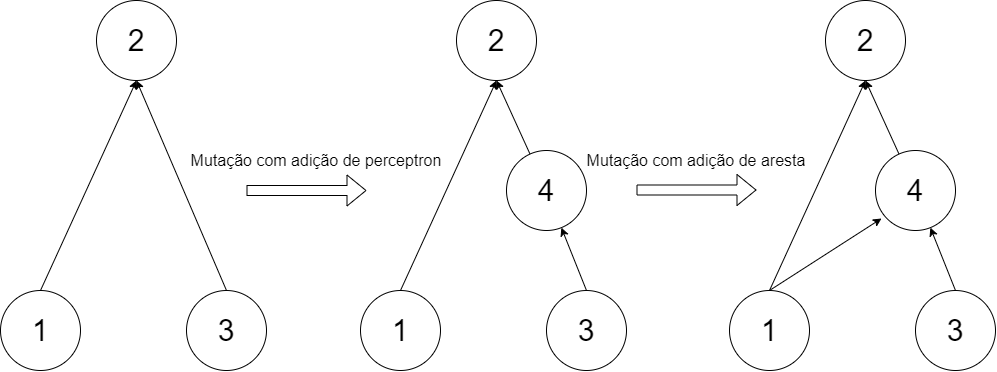
\includegraphics[width=0.7\textwidth]{images/MutaçãoDeTopologias.png}
        \legend{
                Fonte: Autoria Pr{\'o}pria.
        }
\end{figure}

A função \textit{fitness} é definida de acordo com o problema e foca no quão bem as 
topologias da Rede Neural desempenham nas situações onde estão inseridas. 
Durante a reprodução, uma população nova deve ser gerada respeitando 3 regras 
estabelecidas na literatura base do NEAT.

\subsection{Tr{\'i}ade de efici{\^e}ncia}

De acordo com \citeonline{stanley2002}, a eficiência do NEAT é proveniente de um 
tripé que consiste em promover cruzamentos genéticos que não empobreçam a 
capacidade computacional das proles em relação aos pais, proteger inovações 
genéticas por meio do processo de especiação e buscar soluções a partir de 
topologias simples, incrementando-as gradativamente. 

Para que o algoritmo atinja o objetivo de gerar uma reprodução sem que se 
tenha perda na capacidade computacional, a codificação do AG deve assegurar que 
durante o processo de seleção para a reprodução, esta seja feita de maneira correta, 
selecionando as topologias com melhor \textit{fitness} e também garantindo que haja 
pluralidade de características quando selecionando topologias de pior desempenho, 
para que se consiga captar boas qualidades mesmo possuindo um desempenho baixo. Com 
esse processo se faz possível a geração de espécies, abrangendo o 
segundo ponto do tripé proposto por \citeonline{stanley2002}.

A especiação é colocada como um caminho para que os resultados provenientes 
do NEAT sejam completos e capazes de se adaptar em diferentes situações. Observando 
uma geração onde todos possuem as mesmas características com um 
bom desempenho em uma cenário específico, ao alterar a situação em que se 
encontram, a tendência é que todas as topologias demonstrem comportamento 
parecido, que pode ou não encaixar na circunstância proposta. Justamente para evitar essa 
situação, a configuração do AG deve garantir que as topologias de Rede Neural 
pertencentes à população sejam próximas, porém com diferentes qualidades que 
propiciem uma melhor adaptação.

Iniciar uma população de Redes Neurais densas pode ser 
desnecessariamente custoso, pois o algoritmo precisaria de muito tempo para 
otimizar estruturas complexas \cite{stanley2002}. Para evitar tal 
custo elevado, o NEAT inicia suas topologias sem possuir camadas ocultas e com 
arestas de conexão diretas entre entradas e saídas, possibilitando o cruzamento e mutação de 
topologias aleatórias capazes de gerar melhores resultados.

\subsection{Aplica{\c c}{\~a}o no projeto}

Trazendo o NEAT para a situação demonstrada por esse projeto, é possível 
visualizar todos os conceitos supracitados. A simulação no ambiente de carros 
autônomos se dá com cada veículo em questão possuindo sua própria topologia 
inicial simples, sendo esta alterada a cada rodada de simulação com o processo 
de reprodução das topologias de Rede Neural de acordo com as regras do AG. 

O processo de especiação está suscetível a ocorrer, com veículos possuindo 
características diferentes entre si focando no mesmo resultado. Por exemplo, há a 
possibilidade de uma espécie de veículo fazer uma curva à direita de maneira mais 
suave, percorrendo toda a extensão da curva, ao mesmo tempo em que outro 
veículo pode fazer um movimento mais seco e abrupto, somente virando à direita, 
dando uma maior variedade aos indivíduos da população.
